\documentclass[tikz,border=2pt]{standalone}
\usepackage{amsmath,amssymb}
\usepackage{tikz}
\usetikzlibrary{arrows.meta,calc,positioning}

\begin{document}
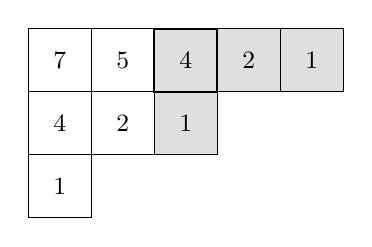
\begin{tikzpicture}[>=Stealth]
  % Global box size and text style
  \def\bs{0.8} % box size in cm
  \tikzset{
    cell/.style = {draw, minimum width=\bs cm, minimum height=\bs cm, inner sep=0pt, outer sep=0pt, anchor=south west},
    num/.style  = {font=\small},
    hookmark/.style = {line width=0.9pt}
  }

  % Grid units scaled by \bs
  \begin{scope}[x=\bs cm,y=\bs cm]
    % Shape λ = (5,3,1): rows y=2 (len 5), y=1 (len 3), y=0 (len 1)

    % --- Shade the hook of the chosen cell (i,j) = (1,3) ---
    % (top row y=2, column 3 -> x=2). Hook = itself + rightwards + downward.
    \fill[gray!25] (2,2) rectangle ++(1,1); % the cell itself
    \fill[gray!25] (3,2) rectangle ++(1,1); % right 1
    \fill[gray!25] (4,2) rectangle ++(1,1); % right 2
    \fill[gray!25] (2,1) rectangle ++(1,1); % down 1

    % Optional: emphasize the chosen (i,j) cell border
    \draw[hookmark] (2,2) rectangle ++(1,1);

    % --- Draw the Young diagram boxes ---
    % Row 1 (top) length 5 at y=2
    \foreach \x in {0,1,2,3,4} { \node[cell] at (\x,2) {}; }
    % Row 2 length 3 at y=1
    \foreach \x in {0,1,2}     { \node[cell] at (\x,1) {}; }
    % Row 3 length 1 at y=0
    \node[cell] at (0,0) {};

    % --- Hook lengths in each cell (λ = (5,3,1)) ---
    % Row 1 (y=2): 7 5 4 2 1
    \node[num] at (0.5,2.5) {7};
    \node[num] at (1.5,2.5) {5};
    \node[num] at (2.5,2.5) {4};
    \node[num] at (3.5,2.5) {2};
    \node[num] at (4.5,2.5) {1};

    % Row 2 (y=1): 4 2 1
    \node[num] at (0.5,1.5) {4};
    \node[num] at (1.5,1.5) {2};
    \node[num] at (2.5,1.5) {1};

    % Row 3 (y=0): 1
    \node[num] at (0.5,0.5) {1};

    % (Optional) label:
    % \node[font=\footnotesize] at (2, -0.8) {$\lambda=(5,3,1)$; hook at $(i,j)=(1,3)$};

  \end{scope}
\end{tikzpicture}
\end{document}
